\section{État de l'art}


\subsection{Les technologies IoT dans les voitures}

\commentaire{introduction}
Selon l’entreprise Objenious \cite{noauthor_revolution_2025}, l’Internet des Objets (IoT) constitue une révolution dans l’industrie automobile en rendant les véhicules plus intelligents et connectés. Depuis l’introduction de la norme européenne eCall en 2018, qui impose un système d’appel d’urgence automatique, les constructeurs ont intégré des technologies IoT pour développer des services innovants. Grâce aux réseaux haut débit comme la 4G et la 5G, les véhicules peuvent désormais collecter, envoyer et recevoir des données en temps réel, interagissant ainsi avec les infrastructures routières, les autres véhicules et les usagers.\\
Le marché mondial de l’IoT dans le secteur automobile, estimé à 115,37 milliards de dollars en 2022, devrait atteindre 975,66 milliards de dollars d’ici 2032, avec un TCAC\footnote{Taux de Croissance Annuel Composé : C’est un indicateur qui permet de mesurer la croissance moyenne d’un marché, d’un chiffre d’affaires ou d’un investissement sur plusieurs années, en tenant compte de l’effet cumulatif d’une année sur l’autre.} de 23,8 \% sur cette période \cite{noauthor_taille_2023}.\\
L’intégration des technologies IoT dans les véhicules permet une communication en temps réel entre les véhicules eux-mêmes, les infrastructures et d’autres dispositifs externes. Cette connectivité vise à améliorer la sécurité, l’efficacité et l’expérience de conduite. Les capteurs embarqués collectent et échangent des données sur les conditions de circulation, la météo, les performances du véhicule et le comportement du conducteur. Ces informations sont exploitées pour la maintenance prédictive, la navigation intelligente et l’optimisation des systèmes de conduite autonome.\\
Par ailleurs, la connectivité IoT facilite l’intégration des smartphones et autres appareils avec les véhicules, offrant ainsi des services tels que la surveillance à distance, le suivi des véhicules et des fonctionnalités d’info-divertissement personnalisées. Ces avancées technologiques redéfinissent le secteur automobile, ouvrant la voie à une mobilité plus sûre, plus intelligente et plus autonome.


\subsubsection{Systèmes de communication et d’échange de données}
\todo{A DÉVELOPPER ?}
"Depuis longtemps une voiture collecte des données, ces données sont collectées via les capteurs et traitées par les calculateurs du véhicule." par Innovauto \cite{donnees_echange}. Les premiers calculateurs électroniques embarqués (ECU) ont été introduits à la fin des années 1970, principalement pour la gestion du moteur. Leur présence s’est progressivement renforcée, et l’utilisation généralisée de capteurs et de calculateurs s’est imposée dans les années 1990 et 2000 avec l’apparition de systèmes comme l’ABS, l’ESP ou encore l’injection électronique. Aujourd’hui, les véhicules modernes intègrent plusieurs dizaines, voire plusieurs centaines de capteurs et de calculateurs, qui assurent le fonctionnement et la sécurité de l’ensemble du véhicule. \\
Les différentes données émises par un véhicule peuvent être \textbf{techniques} (par exemple : état de charge de la batterie, autonomie restante ...), \textbf{usage} (par exemple : type de trajet, style de conduite...) et \textbf{personnelles} (par exemple : titulaire de la carte grise, agenda du conducteur,...).
%cycle de vie de la donnée
Un véhicule autonome échange des données avec son environnement, et ces données suivent un cycle de vie comportant plusieurs étapes :
\begin{figure}[H]
    \centering
    \includegraphics[width=0.8\textwidth]{images/schéma_cycle_vie_donneées.png} 
    \caption{Cycle de vie de la donnée}
\end{figure}
Les étapes du cycle de vie des données doivent respecter le RGPD\footnote{Règlement Général sur la Protection des Données : Il établit un cadre juridique unifié pour la collecte, le traitement et la protection des données personnelles au sein de l’Union européenne} sans être spécifiquement adaptées à la pratique automobile. De plus, si des véhicules sont commercialisés, ils doivent se conformer aux normes de chaque pays, telles que le RGPD en Europe, le Cloud Act aux États-Unis, et le PIPL\footnote{ Personal Information Protection Law : C’est la loi chinoise entrée en vigueur le 1er novembre 2021, qui encadre la collecte, l’utilisation, le stockage et le partage des données personnelles.} en Chine. Voici un exemple comparatif :
\begin{table}[H]
\centering
\caption{Comparaison entre le RGPD (Union européenne) et le PIPL (Chine)}
\begin{tabular}{|p{4cm}|p{5cm}|p{5cm}|}
\hline
\textbf{Critère} & \textbf{RGPD (UE)} & \textbf{PIPL (Chine)} \\ \hline
\textbf{Date d'entrée en vigueur} & 25 mai 2018 & 1er novembre 2021 \\ \hline
\textbf{Champ d'application} & Toutes les organisations qui traitent des données personnelles de résidents de l’UE, peu importe leur localisation. & Toutes les organisations qui traitent des données personnelles de résidents chinois, y compris à l’étranger si cela concerne leurs droits et intérêts. \\ \hline
\textbf{Consentement} & Doit être libre, spécifique, éclairé et univoque. & Doit être clair, volontaire et informé, avec un accord explicite requis dans certains cas (par ex. données sensibles). \\ \hline
\textbf{Principes clés} & Licéité, loyauté, transparence, limitation des finalités, minimisation, exactitude, limitation de la conservation, intégrité, confidentialité. & Finalité claire, minimisation, transparence, sécurité, responsabilité, respect des droits individuels. \\ \hline
\textbf{Droits des individus} & Accès, rectification, effacement, limitation, opposition, portabilité des données. & Accès, copie, correction, suppression, limitation, opposition, explication du traitement. \\ \hline
\textbf{Données sensibles} & Traitement soumis à des conditions strictes (santé, biométriques, opinions politiques...). & Nécessite un consentement explicite et des mesures renforcées (santé, biométriques, localisation, données financières...). \\ \hline
\textbf{Transfert international} & Autorisé vers pays disposant d’un niveau de protection adéquat ou via clauses contractuelles types. & Soumis à une évaluation de sécurité par l'autorité chinoise et, parfois, à une autorisation préalable. \\ \hline
\textbf{Sanctions} & Jusqu’à 20 millions € ou 4\% du chiffre d’affaires annuel mondial (le plus élevé des deux). & Jusqu’à 50 millions CNY (\textasciitilde 7 millions €) ou 5\% du chiffre d’affaires annuel. \\ \hline
\end{tabular}
\end{table}
En résumé, bien que le RGPD et le PIPL partagent un objectif commun de protection des données personnelles, leurs approches diffèrent sur plusieurs points, notamment dans la portée territoriale, le rôle des autorités de contrôle et le niveau de centralisation des obligations. Le RGPD se concentre sur la transparence et le consentement explicite, 
tandis que le PIPL intègre des exigences plus strictes en matière de transfert transfrontalier et un contrôle accru de l’État.\\
Les données collectées par les véhicules autonomes sont considérées comme des données personnelles et doivent être protégées conformément à la réglementation en vigueur d'après la Thèse de Nolwen LE GUENNEC\cite{le_gennec_machine_2023}.\\
La connectivité des véhicules autonomes pose également des problèmes de sécurité, notamment la vulnérabilité aux attaques informatiques. Des questions se posent sur la manière de protéger ces systèmes contre de telles menaces. Comment peut-on sécuriser ces informations sensibles face aux cyberattaques ?\\
Les programmes informatiques consomment de l’énergie et l'impact environnemental de ces technologies doit être pris en compte.\\
Grâce à la technologie IoT, les véhicules peuvent échanger des données. Voici les 3 modes de fonctionnement des STI\footnote{Système de Transport Intelligent} :
\begin{itemize}
    \item \textbf{Communication véhicule à véhicule (V2V)} : Les véhicules équipés de l’IoT échangent des informations telles que leur vitesse et leur position. Cette communication permet de signaler des accidents ou des pannes, aidant les conducteurs à anticiper les problèmes de circulation et à se déplacer plus efficacement.
    \item \textbf{Communication véhicule à infrastructure (V2I)} : Les véhicules connectés interagissent avec des éléments d’infrastructure routière comme les feux de circulation, les lampadaires et les caméras. L’analyse de ces données peut conduire à des ajustements tels que la modification des limites de vitesse ou la facilitation du passage des véhicules de secours, améliorant ainsi la sécurité routière pour tous les usagers.
    \item \textbf{Communication infrastructure au véhicule (I2V)} : Les infrastructures routières transmettent des informations aux véhicules à proximité, permettant l’affichage en temps réel de données pertinentes pour les conducteurs.
\end{itemize}

\begin{figure}[H]
    \centering
    \includegraphics[width=0.9\textwidth]{images/schéma_systeme_communication_donnees.png} 
    \caption{Tableau comparatif du système de communication V2X d'Innovauto}
\end{figure}

La technologie basée sur les opérateurs mobiles permet une communication avec un serveur distant, mais ne prend pas en charge directement la communication entre véhicules et infrastructures : 
\begin{itemize}
    \item Le ITS-G5 (Wi-Fi) fonctionne sur la bande 5,9 GHz et permet une communication locale et directe entre les véhicules, les infrastructures et les piétons.
    \item Le C-V2X (Cellular-V2X) combine les deux approches, offrant à la fois une communication via les réseaux mobiles et une communication directe entre les véhicules et infrastructures.
    \item Le C-V2X est la solution la plus complète, intégrant les avantages des réseaux mobiles et de la communication directe, ce qui le rend plus adapté aux véhicules autonomes et à la gestion du trafic intelligent.
\end{itemize}

\subsubsection{Capteurs et perception environnementale}
L'évolution des véhicules intelligents repose sur des systèmes de capteurs avancés et de perception environnementale. "Un capteur IoT est un dispositif qui mesure une ou plusieurs variables physiques de l'environnement et envoie les données à un réseau ou à une plateforme IoT pour une utilisation ultérieure." selon le site de l'entreprise IoT\cite{iot_capteur}.\\
Ces technologies permettent aux véhicules de collecter, d'analyser et d'interpréter en temps réel leur environnement afin d'améliorer leur utilisation.
Les principaux capteurs utilisés sont les caméras, les radars, les lidars et les ultrasons.
Ces données permettent de :\\
- Détecter les pannes. \\
- Alerter les propriétaires en cas de dysfonctionnement. \\
- Optimiser la maintenance. \\
- Simplifier les procédures de réparation. \\
- Gérer les flottes de véhicules. \\

%Par exemple, Lormauto, un constructeur français spécialisé dans le rétrofit de véhicules, utilise la connectivité cellulaire 4G pour optimiser l’expérience utilisateur. Cette technologie permet de transmettre de grands volumes d’informations et de surveiller l’état de santé des véhicules et de leurs batteries en temps réel.

La perception de l'environnement consiste à analyser et à interpréter les données fournies par les capteurs pour prendre des décisions en temps réel. La décision repose sur des algorithmes avancés d'IA\footnote{Intelligence Artificielle} qui permettent de reconnaître les objets, d'anticiper les comportements et de réagir en conséquence. Ces technologies sont essentielles pour la conduite autonome et la sécurité des usagers de la route, y compris les motards.
Pour cela, il faut combiner plusieurs informations :
\begin{itemize}
    \item Détecter et classer les objets,
    \item Estimer leur vitesse et leur trajectoire,
    \item Anticiper les risques et les collisions,
    \item Améliorer la prise de décision.
\end{itemize}
Les avancées en IA en connectivité comme la 5G et la V2X et en traitement des données continueront d’améliorer la perception environnementale des véhicules permettant ainsi la voie à une mobilité plus sûre.

\subsubsection{Aide à la conduite et systèmes ADAS}
%•Détection des obstacles et freinage automatique.
%•Avertissements de collision et assistance au changement de voie.
Dans un monde où la sécurité routière est une priorité, les systèmes avancés d’aide à la conduite (ADAS) révolutionnent la manière dont les véhicules interagissent avec leur environnement, réduisant ainsi les risques d’accidents et améliorant l’expérience de conduite.
Selon le site du Gouvernement \cite{adas_gouv} "Ces technologies ouvrent la voie à des véhicules de plus en plus automatisés, mais ceux qui en sont équipés ne sont pas des véhicules dits « autonomes ». Les aides à la conduite ne remplacent pas le conducteur et ses obligations. Leur usage s’opère sous la surveillance permanente du conducteur, qui reste responsable de la tâche de conduite et de la maîtrise du véhicule."
\begin{figure}[H]
    \centering
    \includegraphics[width=0.8\textwidth]{images/ADAS_schéma.jpg} 
    \caption{Voiture embarquant des systèmes ADAS\cite{continental_adas}}
\end{figure}


\subsubsection{Analyse des données et prise de décision}
L'entreprise Valeo a conçu un radar Lidar « Scala ». D'après LeParisien \cite{le_parisien_radar_2019}, l'entreprise, en 2020 produit 200 000 exemplaires par an. Cette technologie permet grâce à cette technologie, la voiture peut circuler sans l’intervention d’un conducteur.\\
\commentaire{yann lecun}
Les recherches sur l'utilisation et l'interprétation des données recueillies par les capteurs sont au coeur des sujets depuis quelques années. Yann LeCun, précurseur du deep learning\footnote{L'apprentissage automatique.} nous présente l'interprétation et l'utilisation de données recueillies.
Ce graphe ci-dessous présente la relation entre l’écart de position d’une voiture sur la voie et l’angle du volant pour ramener la voiture au milieu. 

\begin{figure}[H]
    \centering
    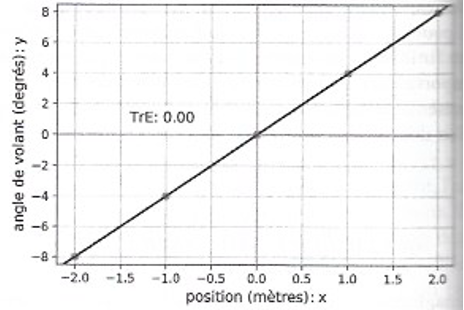
\includegraphics[width=0.7\textwidth]{images/graph1_yannLeCun.png} 
    \caption{Graphe page 88 du livre "Quand la machine apprend".}
\end{figure}
Par exemple, pour une déviation d’un mètre, il faudra incliner le volant de 4 degrés. 
Voici un nouvel exemple de graphique avec de nouvelles données d’entrée :
\begin{figure}[H]
    \centering
    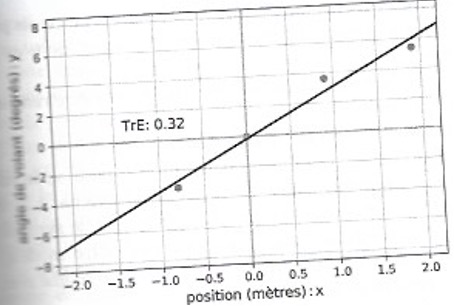
\includegraphics[width=0.7\textwidth]{images/graph2_yannLeCun.jpg} 
    \caption{Graphe page 88 du livre "Quand la machine apprend".}
\end{figure}
La pente passe par trois points sur quatre. Par conséquent, il faut trouver un compromis. On optera donc pour la solution où la droite passe au plus près des quatre points, comme modélisé précédemment. \\
\commentaire{Conclusion Technologie voitures IOT}
En somme, l’IoT révolutionne l’industrie automobile en offrant des véhicules plus sûrs, plus efficaces et mieux entretenus, tout en ouvrant la voie à de nouvelles innovations dans le domaine de la mobilité.\\
\commentaire{conférence}
La mobilité autonome vise à garantir un confort et une fluidité optimaux, ce qui nécessite un système de surveillance pour mesurer diverses variables. Cela se fait principalement par l'utilisation de capteurs embarqués.\\
L'orientation et la direction de la roue jouent un rôle crucial, tout comme la mesure des longitudes et l'utilisation d'unités de mesure inertielle (IMU). La mesure de la vitesse latérale, en revanche, requiert des capteurs très coûteux d'après la conférence\cite{ahmed_ali_synthese_2024} de Sofiane AHMED ALI.\\
Pour réduire le nombre de capteurs nécessaires et, par conséquent, les coûts de développement, on peut utiliser des observateurs\footnote{Observateur : Un outil mathématique ou algorithmique qui permet d’estimer des grandeurs internes d’un système (états) à partir de mesures disponibles et d’un modèle du système.} basés sur des modèles mathématiques pour déterminer les états du véhicule. Cette approche prometteuse présente toutefois des inconvénients, tels que la dynamique latérale du véhicule et les forces latérales agissant sur lui.
L'utilisation de capteurs visuels présente des défis supplémentaires. Ces capteurs peuvent allonger le processus de collecte de données et introduire des délais dans la transmission des images, ayant ainsi un impact majeur sur le système.


\newpage
\subsection{Les défis spécifiques liés à la sécurité des motos}

\subsubsection{Particularités des motos sur la route}
\commentaire{Moins de visibilité et plus de vulnérabilité en cas d’accident.
Dynamique de conduite différente des voitures (accélération rapide, inclinaison dans les virages).}	
Les motos présentent plusieurs particularités sur la route qui impactent leur sécurité et leur interaction avec les autres véhicules.
Une moto, c'est un véhicule de petite taille monté sur deux roues. Cela implique alors qu'elle est encore moins visible, surtout dans les angles morts d'un autre véhicule. Les motos sont agiles, possèdent une forte accélération et leur trajectoire est souvent imprévisible.  Cela accroît le risque de collision, les motos pouvant surprendre les autres usagers de la route. De plus, la configuration du véhicule expose directement le conducteur deux-roues lors d'un accident par son manque de carrosserie. Les conditions météorologiques et la surface de la route jouent un rôle important dans l'adhérence des véhicules. Les conséquences matérielles et corporelles sont beaucoup plus importantes pour un deux-roues car la chute est inévitable.
La puissance de la machine demande beaucoup d'anticipation et une conduite plus exigeante face à tous les dangers.\\

Avec M. Arioui, vice-président de l’innovation et des relations internationales, nous avons abordé la manière dont le regard influence la maîtrise des trajectoires. En effet, le regard est essentiel pour anticiper les dangers et choisir la bonne trajectoire. De plus, tous les facteurs comme l'accélération, quand solliciter\footnote{Solliciter la moto désigne le fait de mettre à contribution, de forcer ou de demander un effort particulier à la machine, par exemple, changer l'inclinaison de la moto de droite à gauche.} la moto influencent la trajectoire. 
La sécurité routière\cite{trajectoire_securite} met en avant cette technique nommée EDSR pour "Entrée, Découverte, Sollicitation de la moto, Reprise de stabilité" permet de prendre un virage en toute sécurité en augmentant le champ de vision afin d'anticiper les dangers. 
\begin{figure}[H]
    \centering
    \includegraphics[width=0.4\textwidth]{etat_art/images/trajectoire_securité.jpg} 
    \caption{Trajectoire de sécurité}
\end{figure}
Ci-dessous, l'importance de l'utilisation des trajectoires de sécurité. Cela permet d'anticiper les évènements qui arrivent en face de nous. Attention, c’est un exemple et bien d’autres facteurs rentrent en jeux en terme de sécurité  (graviers, cyclistes, camions, bus, tracteur...).
\begin{figure}[H]
    \centering
    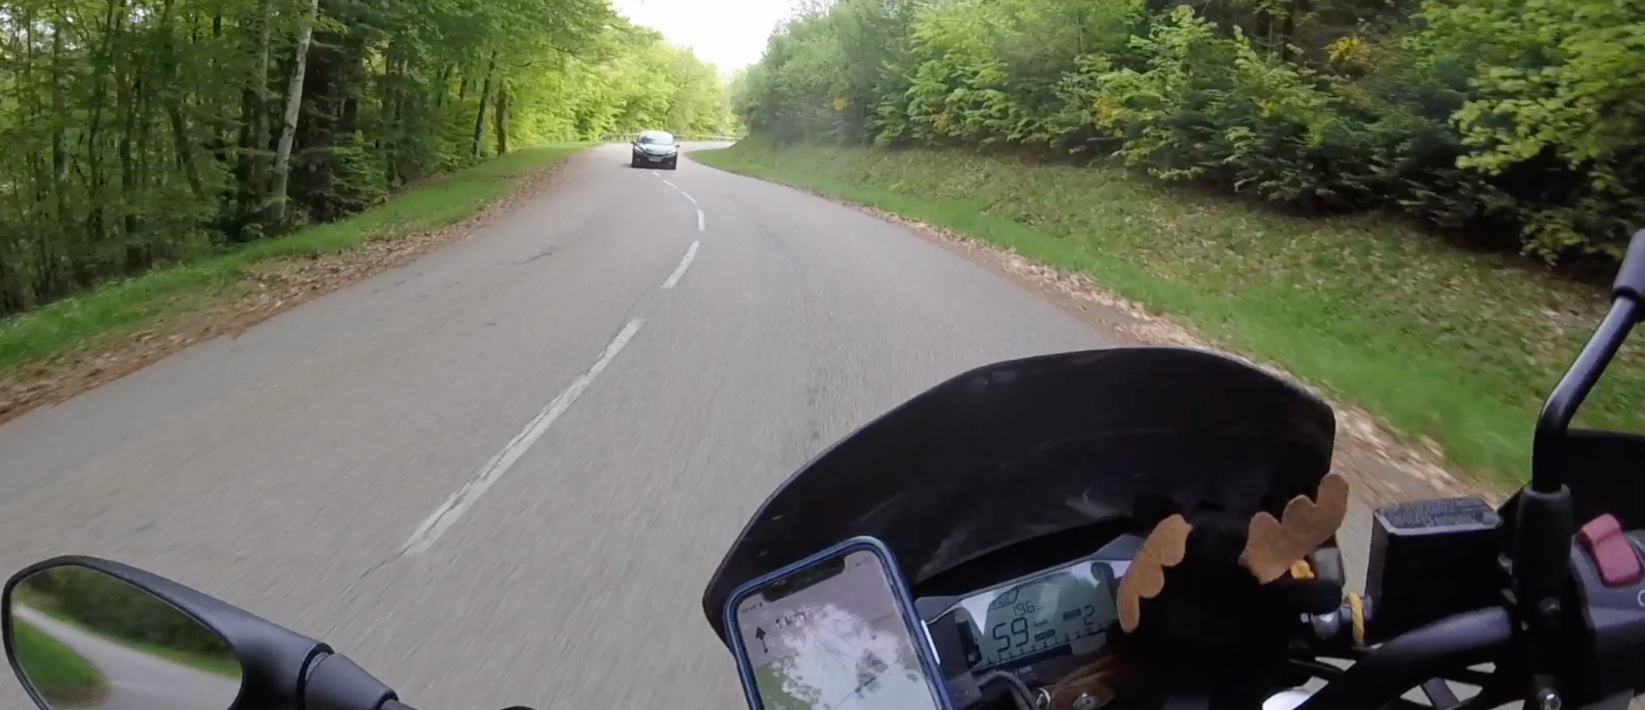
\includegraphics[width=0.6\textwidth]{etat_art/images/morvan.png} 
    \caption{Utilisation de la trajectoire de sécurité à moto}
\end{figure}
Pour mon retour d'expérience, le placement du regard est essentiel pour anticiper ce qu'il arrive en face. En se plaçant externe, cela permet d'agrandir le champ de vision et de pouvoir voir le véhicule qui arrive en face. En se plaçant interne, le champ de vision aurait été réduit et la collision entre les deux véhicules aurait été sûrement inévitable. De plus, la trajectoire de sécurité n'est pas toujours possible, il faut prendre en compte les autres facteurs : la vision (soleil), les véhicules arrivant en face, la qualité de la route...
Cette trajectoire est d'autant plus importante en montagne où les virages sont nombreux et les conditions de circulation imprévisibles. La conduite en montagne nécessite une attention particulière, car les routes peuvent être étroites, sinueuses et parfois glissantes en raison des conditions météorologiques. Les motards doivent donc adapter leur conduite en conséquence, en réduisant leur vitesse et en restant vigilants face aux obstacles potentiels.
\begin{figure}[H]
    \centering
    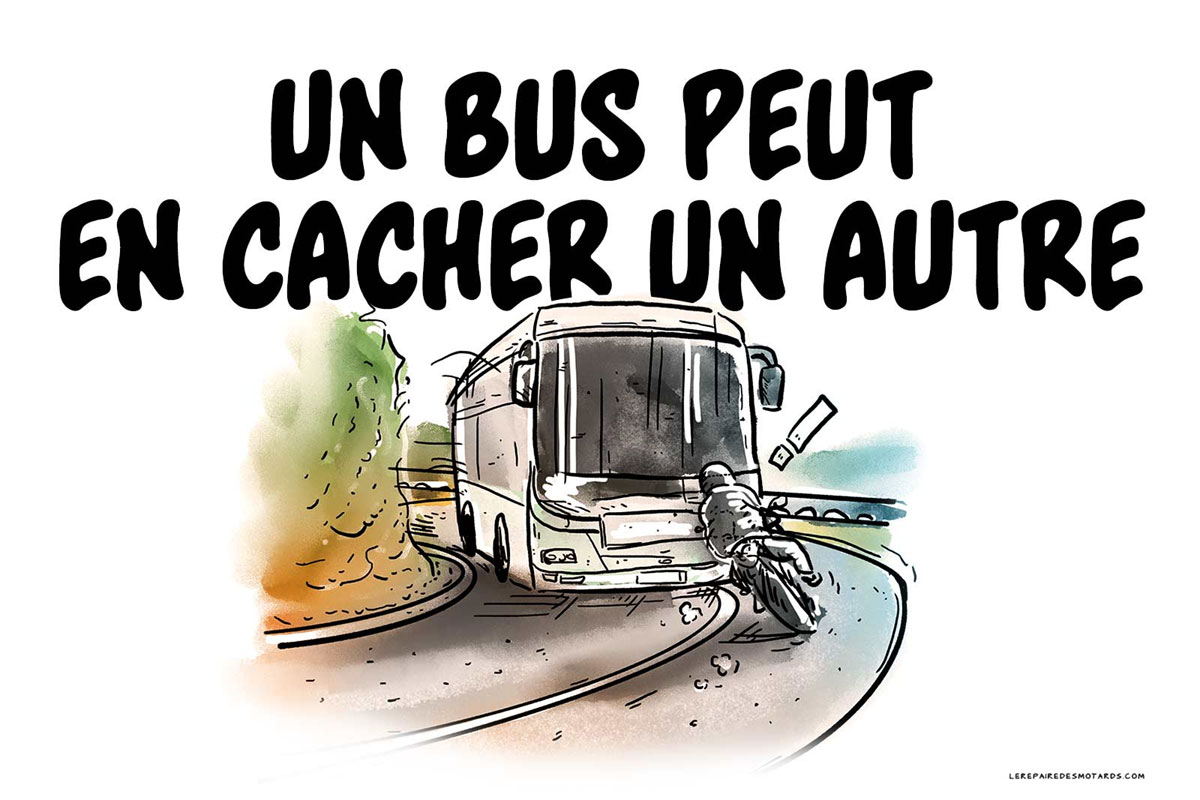
\includegraphics[width=0.6\textwidth]{etat_art/images/trajectoire-route-voie-bus-conduite_hd.jpg} 
    \caption{Illustration de la trajectoire de sécurité en montagne}
\end{figure}
La conduite de nuit constitue un facteur déterminant dans l’analyse des trajectoires. En effet, la réduction de la luminosité naturelle limite fortement les capacités d’anticipation du pilote. Les obstacles, les irrégularités de la chaussée ou encore l’amorce d’un virage sont perçus plus tardivement, ce qui réduit le temps de réaction disponible. La visibilité est restreinte au champ d’éclairage du véhicule, souvent limité, ce qui oblige le motard à adapter sa vitesse et sa position pour conserver une marge de sécurité. 
Ainsi, la nuit impose au motard une adaptation constante de son pilotage, où la prudence et l’anticipation deviennent des éléments clés pour compenser l’absence de repères visuels précis.\\
\vspace{0.5cm}

Ces particularités expliquent pourquoi la sécurité des motos sur la route est un enjeu majeur et nécessite des adaptations spécifiques dans les systèmes de détection et d’assistance à la conduite. 

\subsubsection{Les technologies IoT actuelles pour les motos}
%georide 
Aujourd’hui, de nouvelles marques et applications \cite{iot_accessoire_moto} applications émergent sur le marché de la moto, contribuant à la création d’un écosystème favorable. Celui-ci permet aux propriétaires de deux-roues de s’équiper à moindre coût, notamment grâce à des formules par abonnement. Une des applications que nous pouvons exploiter sur le marché est Georide. Géoride une start-up française qui propose une solution de géolocalisation et de suivi des motos. Grâce à un boîtier connecté, les proches des motards peuvent suivre en temps réel leur trajet. Le boîtier est connecté à un réseau et il a la capacité à détecter une chute puis de contacter l'assistance. 
\begin{figure}[H]
    \centering
    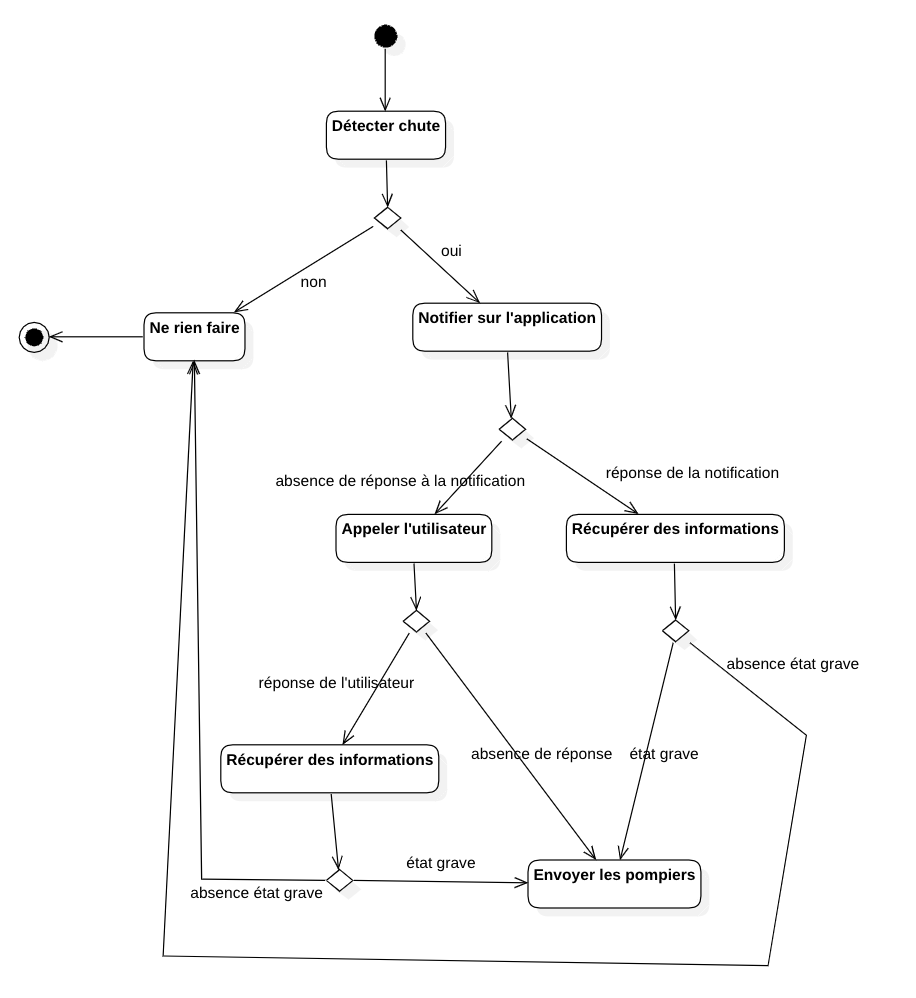
\includegraphics[width=0.8\textwidth]{images/diag_etat_georide.png} 
    \caption{Diagramme d'action du boîtier Géoride concernant la sécurité du motard}
\end{figure}
Ci-dessous, un témoignage d'un utilisateur de l'application Georide à la suite d'un accident à moto. Ce dernier souligne l'importance et le rôle capital que peut avoir la technologie dans la sécurité des motards. Il évoque également la rapidité d'intervention des secours grâce à l'application, ce qui a permis de lui sauver la vie.
\begin{figure}[H]
    \centering
    \includegraphics[width=0.9\textwidth]{etat_art/images/témoignage géoride.png} 
    \caption{Témoignage d'un utilisateur de Georide sur le Discord de l'application réservé pour la communauté}
    \label{temoignage}
\end{figure}
Les dommages corporels sont très violents, même à faible vitesse. La rapidité est un facteur clé dans la survie d'un usager. L’application mobile fournit également des statistiques détaillées sur les performances du véhicule et des alertes en cas de vol ou de panne. Georide propose également des fonctionnalités de partage de trajet, des notifications sur l'entretien de la moto comme le graissage de chaine renforçant ainsi la sécurité et la convivialité de l’expérience de conduite.
\begin{figure}[H]
    \centering
    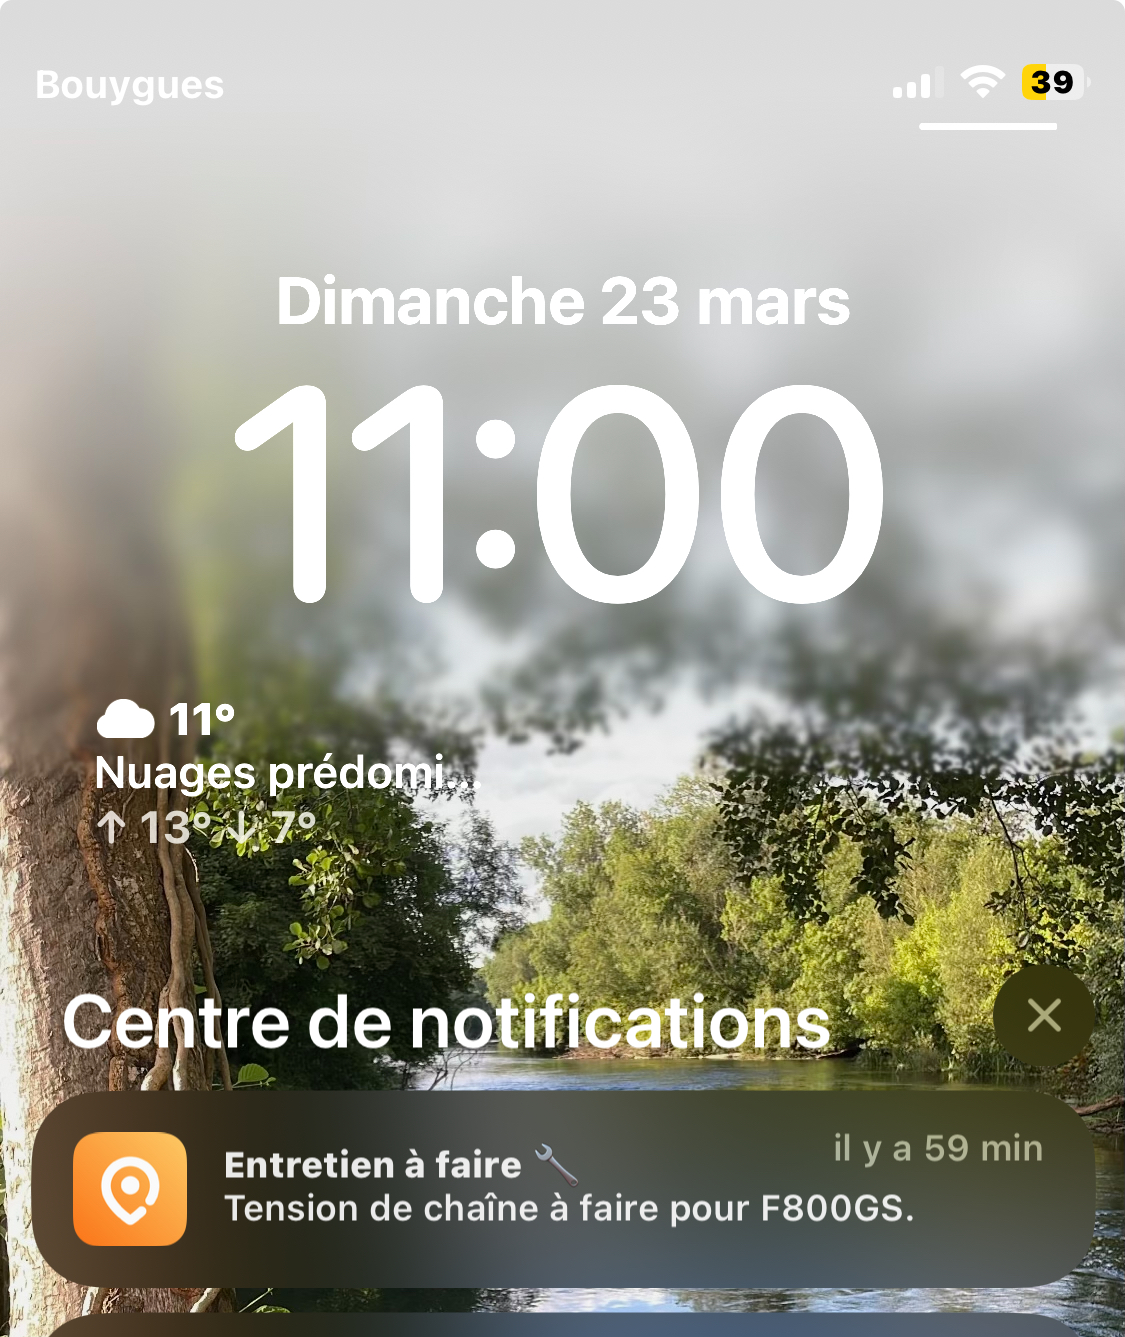
\includegraphics[width=0.5\textwidth]{images/notification_georide.jpg} 
    \caption{Exemple de notification de l'application Georide}
\end{figure}
Pour des motos qui n'ont pas l'option, il est possible d'y ajouter "Live Weel" qui permet de surveiller la pression et la température des pneus. Cela permet de réduire les risques de crevaison.
\vspace{0.5cm}

%Sena, cardo
Des dispositifs de communication sans fil sont également disponibles pour les motards. Des marques comme Sena et Cardo\cite{cardo} proposent des systèmes de communication mains libres qui permettent aux motards de rester connectés tout en conduisant. Ces appareils se fixent sur le casque et offrent des fonctionnalités telles que la communication intercom, la musique en streaming et les appels téléphoniques. Ils sont compatibles avec les smartphones et les systèmes de navigation, améliorant ainsi la sécurité et le confort des motards sur la route. Les dernières mise à jour concernent la détection de collision. Concernant le Packtalk Pro de chez Cardo, il est équipé de capteurs qui permettent de détecter une chute et d'envoyer un message d'urgence à un contact prédéfini.\\
%application
D'autres technologies sont plus accessibles comme celle qui est liée au téléphone. En effet, il existe des applications mobiles qui permettent de suivre son trajet, de partager sa position en temps réel et de recevoir des alertes en cas de danger. Ces applications sont souvent gratuites et faciles à utiliser et peuvent être prises en charge par les assurances: c'est le cas de Liberty Rider \cite{liberty_rider}. Cette application utilise les capteurs du smartphone pour détecter les chutes et envoyer automatiquement un message d'alerte à un contact d’urgence. Elle propose également des fonctionnalités de navigation, prévention des virages dangereux, de partage de trajet et de statistiques de conduite, améliorant ainsi la sécurité et la convivialité de l’expérience de conduite. D'autres applications comme Calimoto, 68 Degrés sont également disponibles et offrent des fonctionnalités similaires pour les motards.\\
\vspace{0.5cm}

%BMW
Pour des motos plus modernes, par exemple, BMW propose des motos connectées\cite{bmw_adas}. La moto est équipée de l’option « Connectivity » qui permet de connecter le smartphone à la moto via Bluetooth. L’écran TFT affiche les informations de navigation, les appels téléphoniques et la musique en streaming. La moto peut aussi être contrôlée via l’application mobile BMW Motorrad Connected, offrant des fonctionnalités de suivi, de maintenance et de partage de trajet. Ces technologies améliorent la sécurité et le confort des motards en leur permettant de rester connectés tout en conduisant.
%ADAS MOTO
Concernant les systèmes ADAS des motos\cite{moto_adas}, il y a des systèmes de freinage ABS,\footnote{Évite le blocage des roues.} de contrôle de traction et de suspension électronique qui sont de plus en plus courants sur les motos modernes. Ces technologies améliorent la stabilité, la maniabilité et la sécurité des motards en ajustant automatiquement les paramètres du véhicule en fonction des conditions de conduite. "De plus, tous les ADAS sur les voitures ne sont pas compatibles et ne seront pas d’une grande utilité sur les motos." d'après l'article de Moto-Net \cite{moto_adas}.
D'après une étude britannique, la technologie ADAS permet de réduire de 20 à 30\%\cite{moto_aras} les accidents de la route. Cependant, ces systèmes ne sont pas encore généralisés sur les motos et leur efficacité dépend de leur intégration et de leur compatibilité avec les spécificités de la conduite à deux-roues. La technologie équivalente à ADAS et ARAS\footnote{Advanced Rider Assistance System} est en cours de développement pour les motos et devrait être déployée dans les prochaines années.
Selon Geoff Liersch, président de la division Deux-roues et sports motorisés chez Bosch, "nous voulons améliorer la sécurité sans retirer le plaisir de la conduite"\cite{aras_bosh}.
Le système ARAS utilise des radars avant et arrière qui communiquent en permanence avec l’Unité de contrôle du moteur (ECU) et divers capteurs.

\begin{figure}[H]
    \centering
    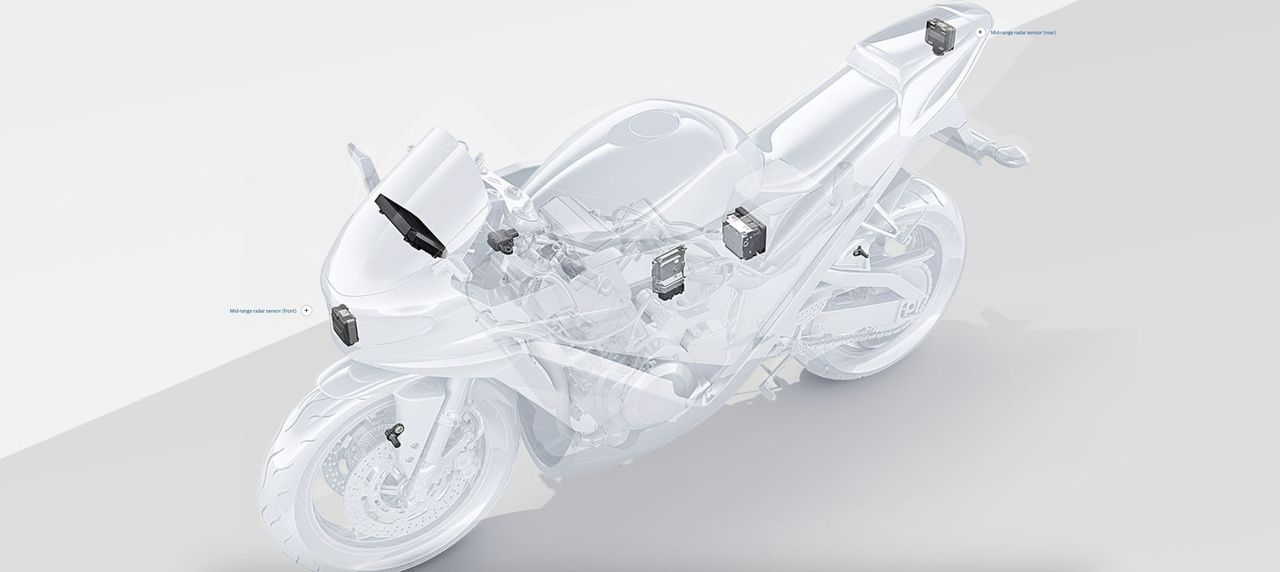
\includegraphics[width=0.7\textwidth]{images/aras_moto.jpeg} 
    \caption{Moto avec la technologie ARAS.}
\end{figure}

%poursuivre avec la suite des tecnhologie
%radar adaptatif
Les radars adaptatifs, déjà utilisés dans l’automobile, font progressivement leur apparition sur les motos haut de gamme. Ce système utilise des capteurs radar pour :
\begin{itemize}
    \item Maintenir une distance de sécurité avec les véhicules qui précèdent.
    \item Avertir le conducteur en cas de risque de collision.
    \item Ajuster le freinage en fonction de l'inclinaison.
    \item Adapter automatiquement la vitesse et la distance de freinage.
    \item Détection d'angles morts.
\end{itemize}
Des constructeurs comme Ducati, BMW et KTM intègrent désormais ce type de radar sur certains modèles, améliorant ainsi l’expérience de conduite, notamment sur autoroute.

%perspectives
Plusieurs nouvelles aides et alertes sont en cours de développement pour les motos. Parmi elles, on retrouve :
\begin{itemize}
    \item Group Ride Assist : Aide à la conduite en groupe.
    \item Régulateur de vitesse adaptatif + Stop and Go : Maintien automatique de la distance de sécurité.
    \item Emergency Brake Assist: Illustré par la Figure~\ref{detecteuravant} est un freinage d’urgence en cas de risque de collision.
\end{itemize}

\begin{figure}[H]
    \centering
    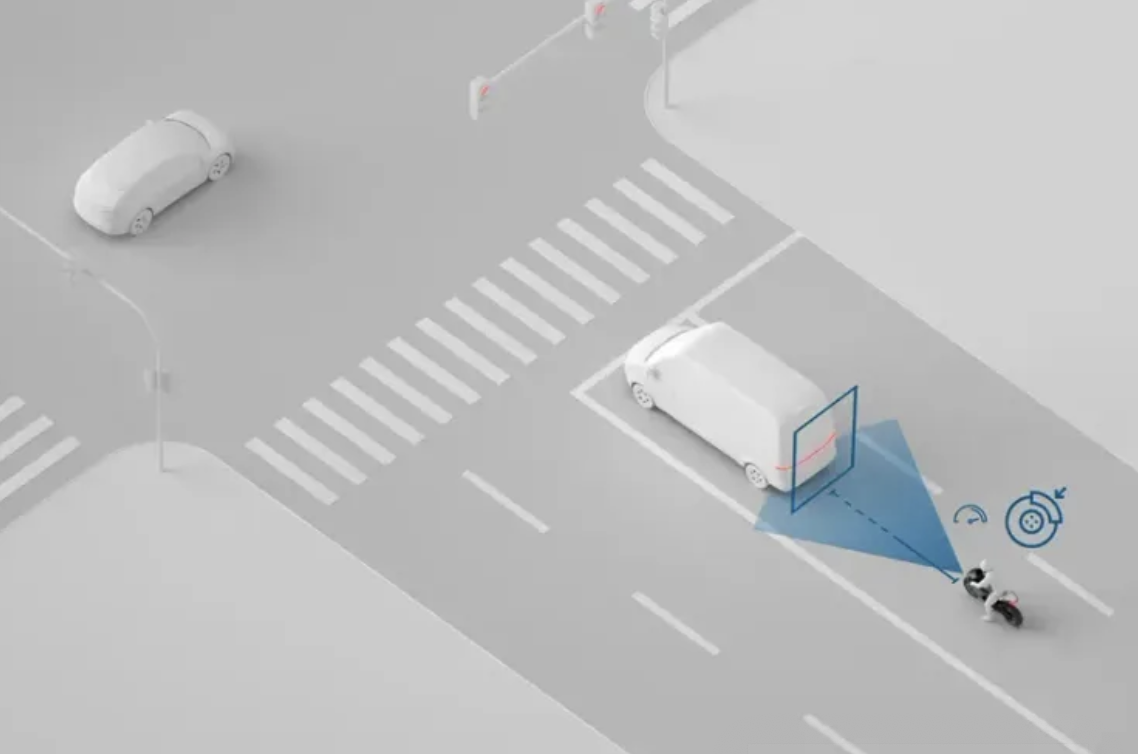
\includegraphics[width=0.7\textwidth]{images/ktm_detecteur_dev.png} 
    \caption{Moto avec la technologie ARAS pour un freinage d'urgence.}
    \label{detecteuravant}
\end{figure}
- Rear Collision Warning: Illustré par la Figure~\ref{detecteurarriere}, il détecte si un véhicule s'approche trop près par l'arrière et active les feux de détresse en cas de risque de collision. 
\begin{figure}[H]
    \centering
    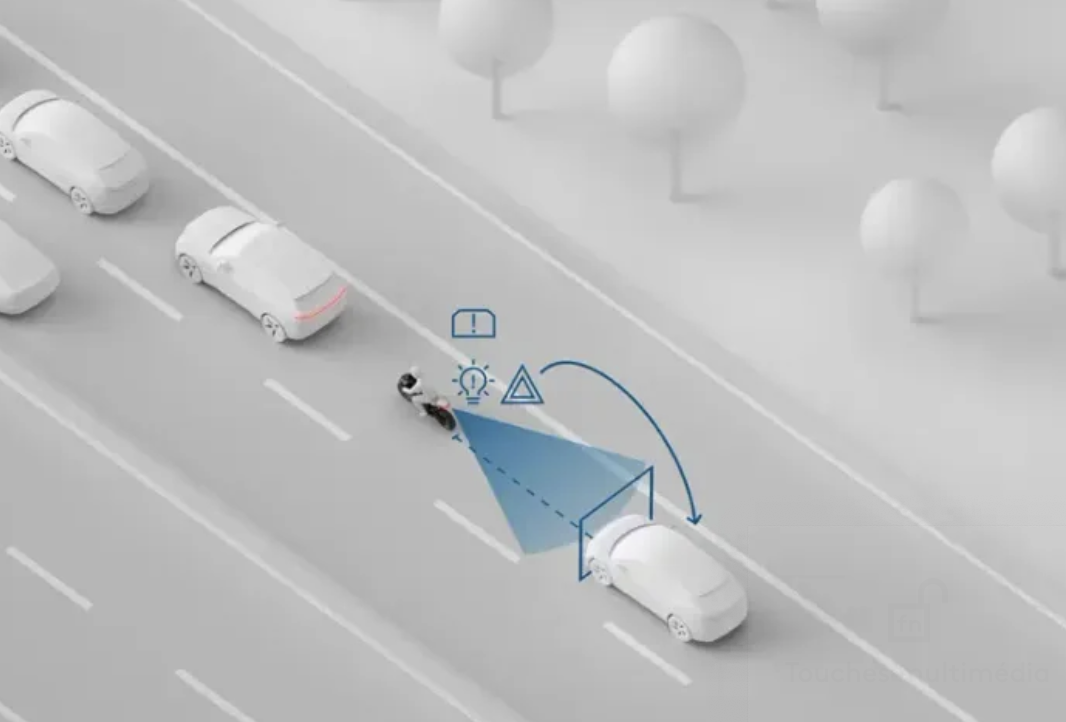
\includegraphics[width=0.7\textwidth]{images/ktm_detecteur.png} 
    \caption{Moto avec la technologie ARAS pour alerter en cas de collision arrière.}
    \label{detecteurarriere}
\end{figure}

"L'objectif est d'avoir cette technologie pour une dizaine d'euros par moto. Cela pourrait réellement avoir un impact significatif sur la réduction des accidents." d'après Geoff Liersch.\\
%possibiliter de continuer les gaz lors de glissade
%abs spécifique moto

%moto autonomes bmw -> A REVOIR
Les motos autonomes sont en cours de développement, avec des prototypes. BMW Motorrad a présenté lors du Consumer Electronic Show 2019 (CES) à Las Vegas \cite{moto_autonome} un modèle de moto autonome capable de se déplacer sans pilote. Ce prototype, basé sur la BMW R 1200 GS, utilise des capteurs et des caméras pour détecter son environnement et naviguer en toute sécurité. Il est capable de démarrer, d’accélérer, de freiner et de tourner sans intervention humaine. 
Ce modèle intègre des technologies avancées telles que la conduite autonome, la connectivité et l’intelligence artificielle. Il est équipé de capteurs et de caméras pour détecter l’environnement et ajuster automatiquement la conduite en fonction des conditions de circulation. La moto est également dotée d’un système de stabilisation qui permet de maintenir l’équilibre même à l’arrêt, offrant ainsi une expérience de conduite plus sûre et plus confortable.

\begin{figure}[H]
    \centering
    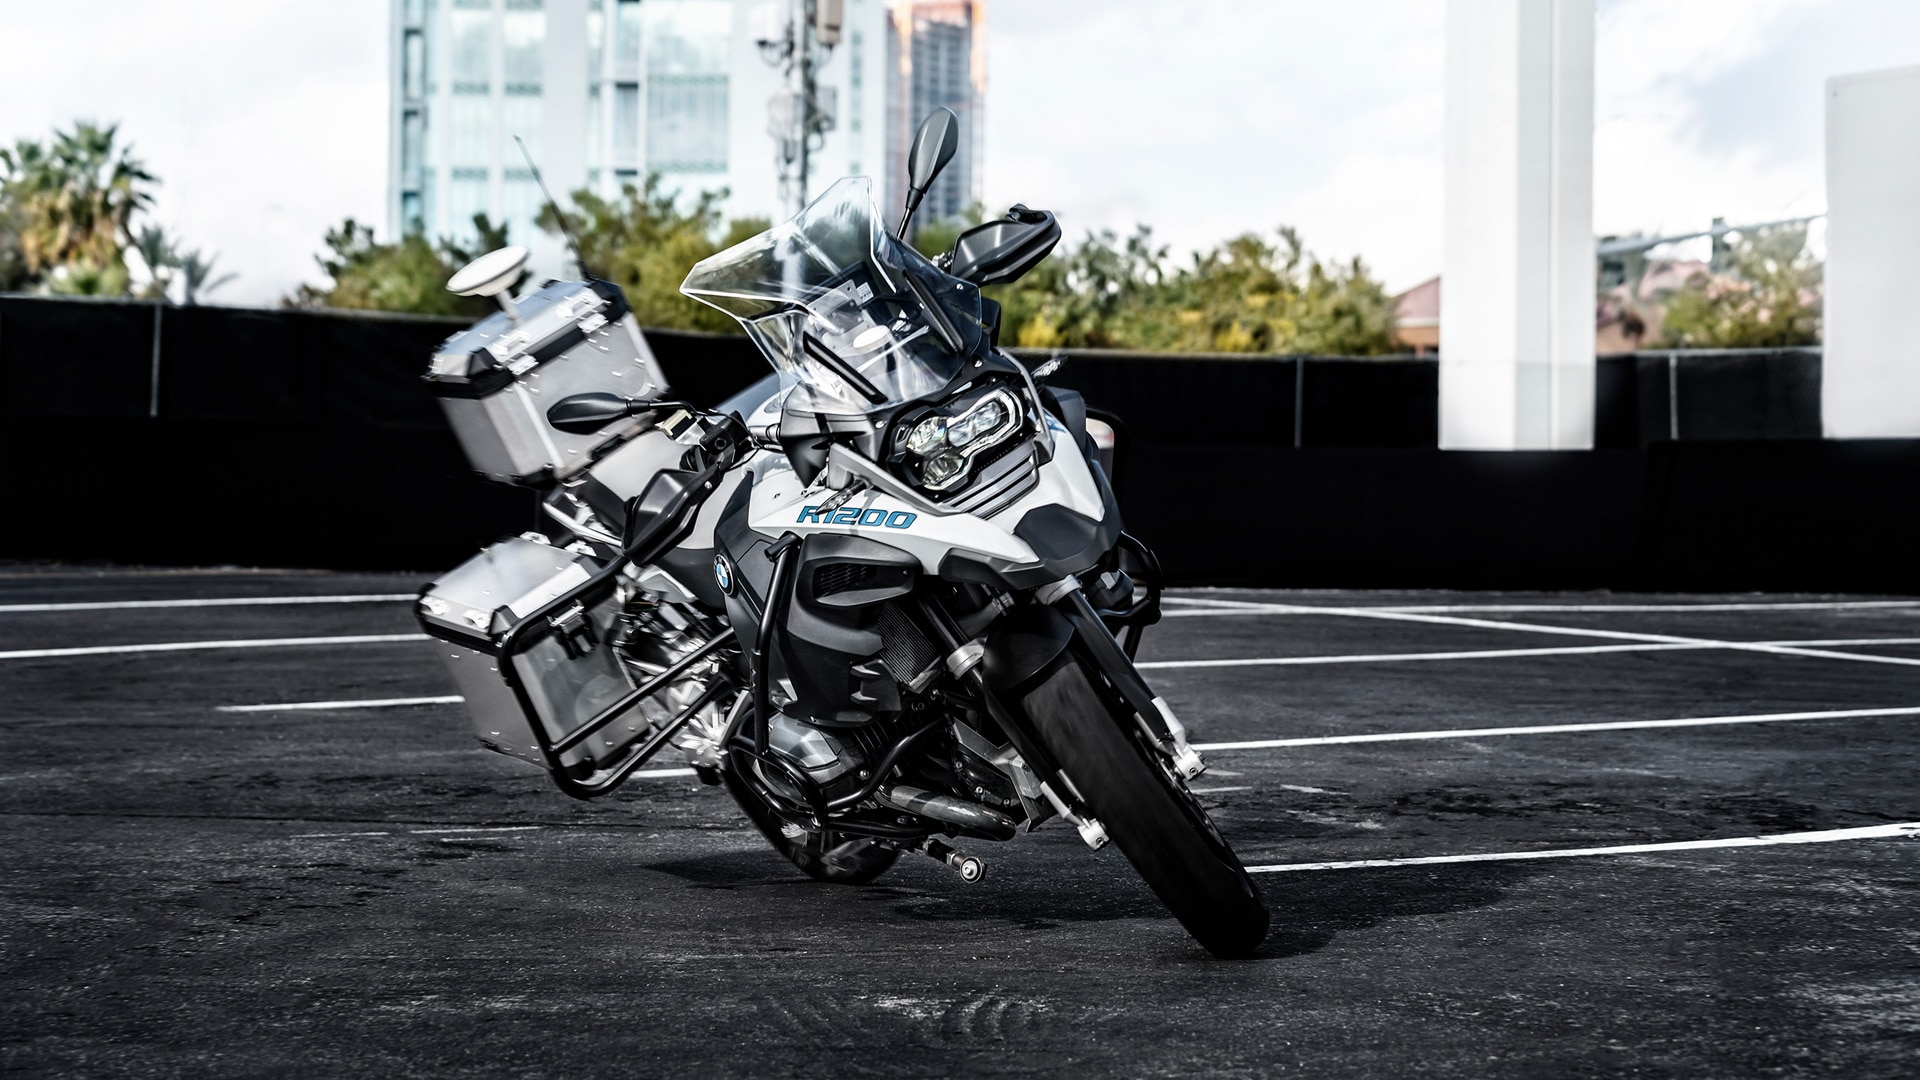
\includegraphics[width=0.7\textwidth]{etat_art/images/bmw.jpeg} 
    \caption{Moto R1300 GS autonome de BMW (2019)}
\end{figure}


\commentaire{Conclusion}
L’intégration de ces technologies dans les motos modernes montre que l’innovation continue d’évoluer pour protéger les motards. Entre les radars adaptatifs, la gestion des gaz en cas de perte d’adhérence et l’ABS spécifique, ces avancées offrent une meilleure stabilité, un freinage plus efficace et une anticipation des dangers sur la route. L’avenir pourrait encore voir l’émergence de nouvelles solutions, comme la communication V2X (Véhicule à Tout) pour améliorer l’interaction entre motos, voitures et infrastructures routières.\\
Avec ces innovations, la moto de demain ne sera pas seulement plus rapide et plus performante, mais surtout plus sûre et plus intelligente. 

\subsubsection{L'exploitation des données pour les motos}
Avec l’essor des technologies embarquées et connectées, les motos modernes génèrent un volume croissant de données, dont l’analyse permet d’améliorer la sécurité, la maintenance et l’expérience de conduite.
Selon Bosch, les systèmes d’assistance basés sur le radar pourraient prévenir un accident de moto sur six \cite{aras_bosh_site_off}, en réagissant plus rapidement que le pilote dans des situations critiques. \\
Des projets comme Dymoa (Cerema) exploitent les données collectées lors des trajets réels pour mieux comprendre les risques propres aux deux-roues et adapter les politiques de sécurité routière.\\
Au sein de Kappa Santé, où j’effectue mon alternance, la sécurité et la confidentialité des données personnelles sont considérées comme essentielles. Des formations obligatoires sur le RGPD sont mises en place afin de sensibiliser les employés à ces enjeux. Cette exigence de rigueur en matière de sécurité m’a permis de mieux appréhender les enjeux liés à la collecte et à l’utilisation des données dans d’autres domaines, comme celui des motos connectées. Il est donc essentiel que les données générées par ces véhicules soient traitées avec le même niveau d’exigence : elles doivent être anonymisées, sécurisées et utilisées de manière responsable afin d’éviter toute fuite ou dérive dans leur exploitation.



\subsubsection{Freins des technologies IoT actuelles pour les motos}
\commentaire{Problèmes de détection par les capteurs des voitures autonomes.
	Communication insuffisante entre motos et véhicules connectés.
	Difficultés d’adaptation des infrastructures intelligentes aux besoins des motards.}

\commentaire{Problème de détection}
Le progrès côté deux-roues est très intéressant et évolue de façon significative.
La Verge TS Ultra est une moto électrique \cite{lenoir_cette_2024} haut de gamme intégrant des technologies avancées pour assurer une sécurité maximale à son pilote. Présentée lors du CES 2024, cette superbike est équipée du système Starmatter Vision, qui comprend six caméras et deux radars haute résolution, offrant une vision à 360 degrés de son environnement. Grâce à l’intelligence artificielle et au machine learning, la TS Ultra analyse en temps réel les risques potentiels et alerte le conducteur, notamment lors des changements de voie. Un écran agrandi sur le réservoir affiche des informations claires, comme la vue arrière lors de l’activation du clignotant. Côté performances, la moto à un moteur de plus de 204 chevaux, permettant une accélération de 0 à 100 km/h en 2,5 secondes. La Verge TS Ultra est disponible à partir de 54 880 euros.
Les technologies qu'embarquent les motos sont à la pointe mais coûtent très chères et ne sont pas encore accessibles à tous.\\
%yamaha
Yamaha, en collaboration avec Netflix, a donné vie à la moto futuriste Y/AI \cite{texier_quand_2024} , initialement imaginée dans la série animée “Tokyo Override”. Ce prototype a été exposé au Motor Expo 2024 en Thaïlande, illustrant la vision de Yamaha sur l’intégration de l’intelligence artificielle dans les motos de demain.\\

\commentaire{moto electrique}
Avec Mr Arioui, vice-président de l’innovation et des relations internationales, nous avons également abordé le sujet des motos électriques. Prenons l'exemple des voitures électriques.
D'après le site Ilek \cite{voiture_electrique}, le moteur électrique "Celui-ci est capable de fournir un couple instantané\footnote{Un couple instantané c’est la mesure du couple à un moment donné qui peut varier en fonction du régime moteur, de la position du piston ou de la charge appliquée.} pour des accélérations fluides et dynamiques". Les voitures électriques ont les mêmes comportements que les motos électriques. Elles sont puissantes, réagissent instantanément. Leur couple\footnote{Plus un moteur est coupleux (qui possède du couple), plus sa capacité à tirer le poids total de la voiture ou d'une moto sera grande.} est élevé.
À la suite d’un échange avec Monsieur Arioui, il ressort que les motos électriques présentent un comportement radicalement différent de celui des motos thermiques. En effet, la puissance est délivrée de manière instantanée, sans aucun temps de latence entre l’action sur l’accélérateur et la réaction de la moto. Ce mode de fonctionnement requiert une phase d’adaptation de la part du motard, tant en termes de maîtrise que d’anticipation des réactions de la machine. Cela demande une adaptation du motard. Une étude présentée lors de la 3ème réunion  \cite{reunionProjet2025} à Nantes a démontré que, selon les usagers, les performances des motos électriques équivalentes à 125 cc seraient comparables à celles de modèles thermiques de 600 cc. La question soulevée est la suivante: "Faudrait-il un permis spécifique pour les motos électriques ?".
Il a été souligné que de nombreux motards privilégient le mode « économie ». Contrairement à ce que son nom laisse penser, ce choix n’est pas uniquement motivé par la volonté de réduire la consommation d'énergie. En réalité, ce mode est souvent utilisé pour abaisser la puissance délivrée et limiter le couple disponible, ce qui rend la moto plus souple, plus "facile à contrôler" et moins dangereuse. 
De plus, le poids de la batterie est important et cela change totalement le comportement de la moto. Ce sont des points à prendre en considération pour la technologie de demain.
Une autre étude a été menée et présentée\cite{reunionProjet2025} sur le retour sensoriel de la vitesse des motards de moto électrique. Cette expérience a été réalisée sur un simulateur. Les différentes expériences ont été réalisées avec ou sans vibration moteur, avec ou sans son... Une expérience avec l'absence visuelle montre une sur estimation de la vitesse. Par exemple, pour une vitesse de 50 km/h, les participants estiment la vitesse à environ plus de 65 km/h. Sans l'audition, la perception de la vitesse est faussée. Pour conclure cette étude, les étudiants ont noté que le visuel représente 41\%, le bruit du moteur représente 21\% enfin, la vibration, 14\%. Le défi ici est d'améliorer les zones d'attention. La décélération d'une moto thermique est de 3,8 km/h contre 5,5 km/h pour une moto thermique.
\vspace{0.5cm} %conclusion

\commentaire{transition}
Les motos électriques intègrent de plus en plus de technologies connectées mais leur adoption peut être freinée par la mentalité de certains motards, encore attachés à une approche plus traditionnelle de la conduite. \\
\vspace{0.5cm}

\commentaire{la mentalité}
D'après une étude réalisée par « The American Automobile Association (AAA) »\cite{consumer_skepticim} en Janvier 2022, il y a 85\% de la population interrogée exprime leur inquiétude, leur peur face à la technologie des voitures autonomes. En effet, cette technologie doit encore faire ses preuves bien que des résultats soient prometteurs.\\
De plus, les médias et les réseaux sociaux ont un impact important sur la perception de la technologie des voitures autonomes. Les accidents impliquant des voitures autonomes sont largement médiatisés et suscitent des débats sur la sécurité et la fiabilité de ces véhicules. Les constructeurs automobiles et les autorités doivent donc communiquer de manière transparente et pédagogique pour rassurer les usagers et favoriser l’adoption de ces technologies.\\
\vspace{0.5cm}

\commentaire{les accidents}
Les réseaux sociaux nous informent en temps réel des événements qui se déroulent dans notre pays ou à travers le monde. 
Récemment, j'ai lu un article (Annexe~\ref{articlevoiture}) daté du jeudi 1er août 2024, relatant un incident survenu en avril dernier. Il s'agit d'un motocycliste de 28 ans, percuté par une voiture en conduite autonome, une Tesla Model S de 2022. Selon les données recueillies, la voiture aurait effectué une embardée après avoir perçu un bruit, ce qui a conduit à la collision. Le fabricant rappelle que ces véhicules ne sont pas entièrement autonomes et que le conducteur doit toujours être prêt à reprendre le contrôle en cas de problème. Selon l'Administration de la sécurité routière des États-Unis, 75 autres accidents impliquant des voitures autonomes ont été recensés. 
La semaine dernière, Elon Musk, PDG de Tesla, a déclaré que d'ici la fin de l'année, les systèmes de "conduite autonome" devraient être capables de fonctionner sans la supervision constante de son conducteur.
\commentaire{limite juridiques}
En cas d'accident, les lois concernant l'intégration d'aide à la conduite est complexe. Nous pouvons nous demander si les règles seront les mêmes que celles soumises aux voitures. Un décret de 2021 précise que si le conducteur respecte les conditions d’utilisation, il peut être dégagé de responsabilité pénale. Le constructeur devient alors pénalement responsable. Toutefois, le conducteur doit rester prêt à reprendre le contrôle lorsqu’il lui est demandé. Selon  Maître Sharon Bensemhoun-Gonzalez sur son site\cite{avocat}, les véhicules autonomes, aujourd’hui utilisés à divers niveaux d’autonomie (jusqu’au niveau 3 selon la norme SAE), soulèvent d’importantes questions en cas d’accident, notamment concernant l’attribution de la responsabilité entre conducteur, constructeur, ou fournisseur de logiciel. Le cadre juridique français reste flou en 2025, malgré les réflexions en cours au niveau européen. Chaque accident nécessite une analyse au cas par cas, souvent complexe pour les victimes. L’indemnisation reste un droit fondamental, notamment via la loi Badinter (1985), et ne peut être remise en question par l’innovation technique.\\
Maître Gonzalez distingue plusieurs situations possibles:
\begin{itemize}
    \item Erreur logicielle (par exemple Un freinage inapproprié par le système autonome)
    \item Défaillance d’un capteur (mauvaise perception de l’environnement)
    \item Inaction du conducteur obligé de reprendre la main 
\end{itemize}
Les responsables peuvent être :
\begin{itemize}
    \item Conducteur : responsabilité civile via l’assurance, même si son intervention n’était pas nécessaire en continu.
    \item Constructeur ou fournisseur : en cas de défaut technique ou vice, une responsabilité contractuelle ou liée à la responsabilité du produit peut être recherchée.
    \item Responsabilité pénale : possible en cas de négligence, désactivation de dispositifs de sécurité ou défaut d’entretien volontaire.
\end{itemize}
Enfin, la victime peut porter plainte ou bien établir un procès-verbal, réaliser des expertises (médicales, matérielle), demander une indemnisation et ou engager une action envers le constructeur. L'utilisation de boîtes noires sont utiles pour l’attribution des faits après accident. L'article\cite{tesla_condamnation} du 1er août 2025, un jury en Floride a condamné Tesla à ~243 M\$ dans un dossier d’accident mortel lié à « Autopilot ». Ce n’est pas du droit UE, mais c’est souvent cité en Europe car il illustre la façon dont des preuves logicielles et de conception sont discutées.\\
Même si l'évolution et le progrès de cette technologie impressionnent et présentent de bons résultats, la technologie montre de nombreuses limites et n'est pas totalement au point.

\newpage
\subsection{Conclusion}
Bien que l’IoT offre de nombreuses opportunités pour améliorer la sécurité et l’efficacité des transports, il présente également des limites et des défis à relever. Ces limites peuvent être liées à la technologie, la réglementation, la sécurité et à la confidentialité des données.\\
Chaque pays a sa propre réglementation et il est difficile de mettre en place une norme commune. Les constructeurs doivent donc s'adapter à chaque marché et respecter les lois en vigueur.\\
La sécurité des données est un enjeu majeur pour les véhicules connectés. Les données collectées par les capteurs et les systèmes embarqués peuvent être sensibles et nécessitent une protection adéquate contre les cyberattaques et les violations de la vie privée.\\
Enfin, l'interopérabilité entre les différents systèmes et véhicules est essentielle pour garantir une communication efficace et une coordination optimale entre les usagers de la route. Les technologies IoT offrent des solutions pour relever ces défis, mais leur mise en œuvre nécessite une collaboration étroite entre les constructeurs, les autorités et les utilisateurs pour garantir une mobilité plus sûre, plus intelligente et plus durable.
Pour conclure, chaque véhicule a des besoins spécifiques et le défi est de trouver des solutions adaptées à chaque type de véhicule. Les technologies IoT offrent des opportunités pour répondre à ces enjeux.\\